\subsection{Kontextdiagramm}
\begin{figure}[h]
    \centering
    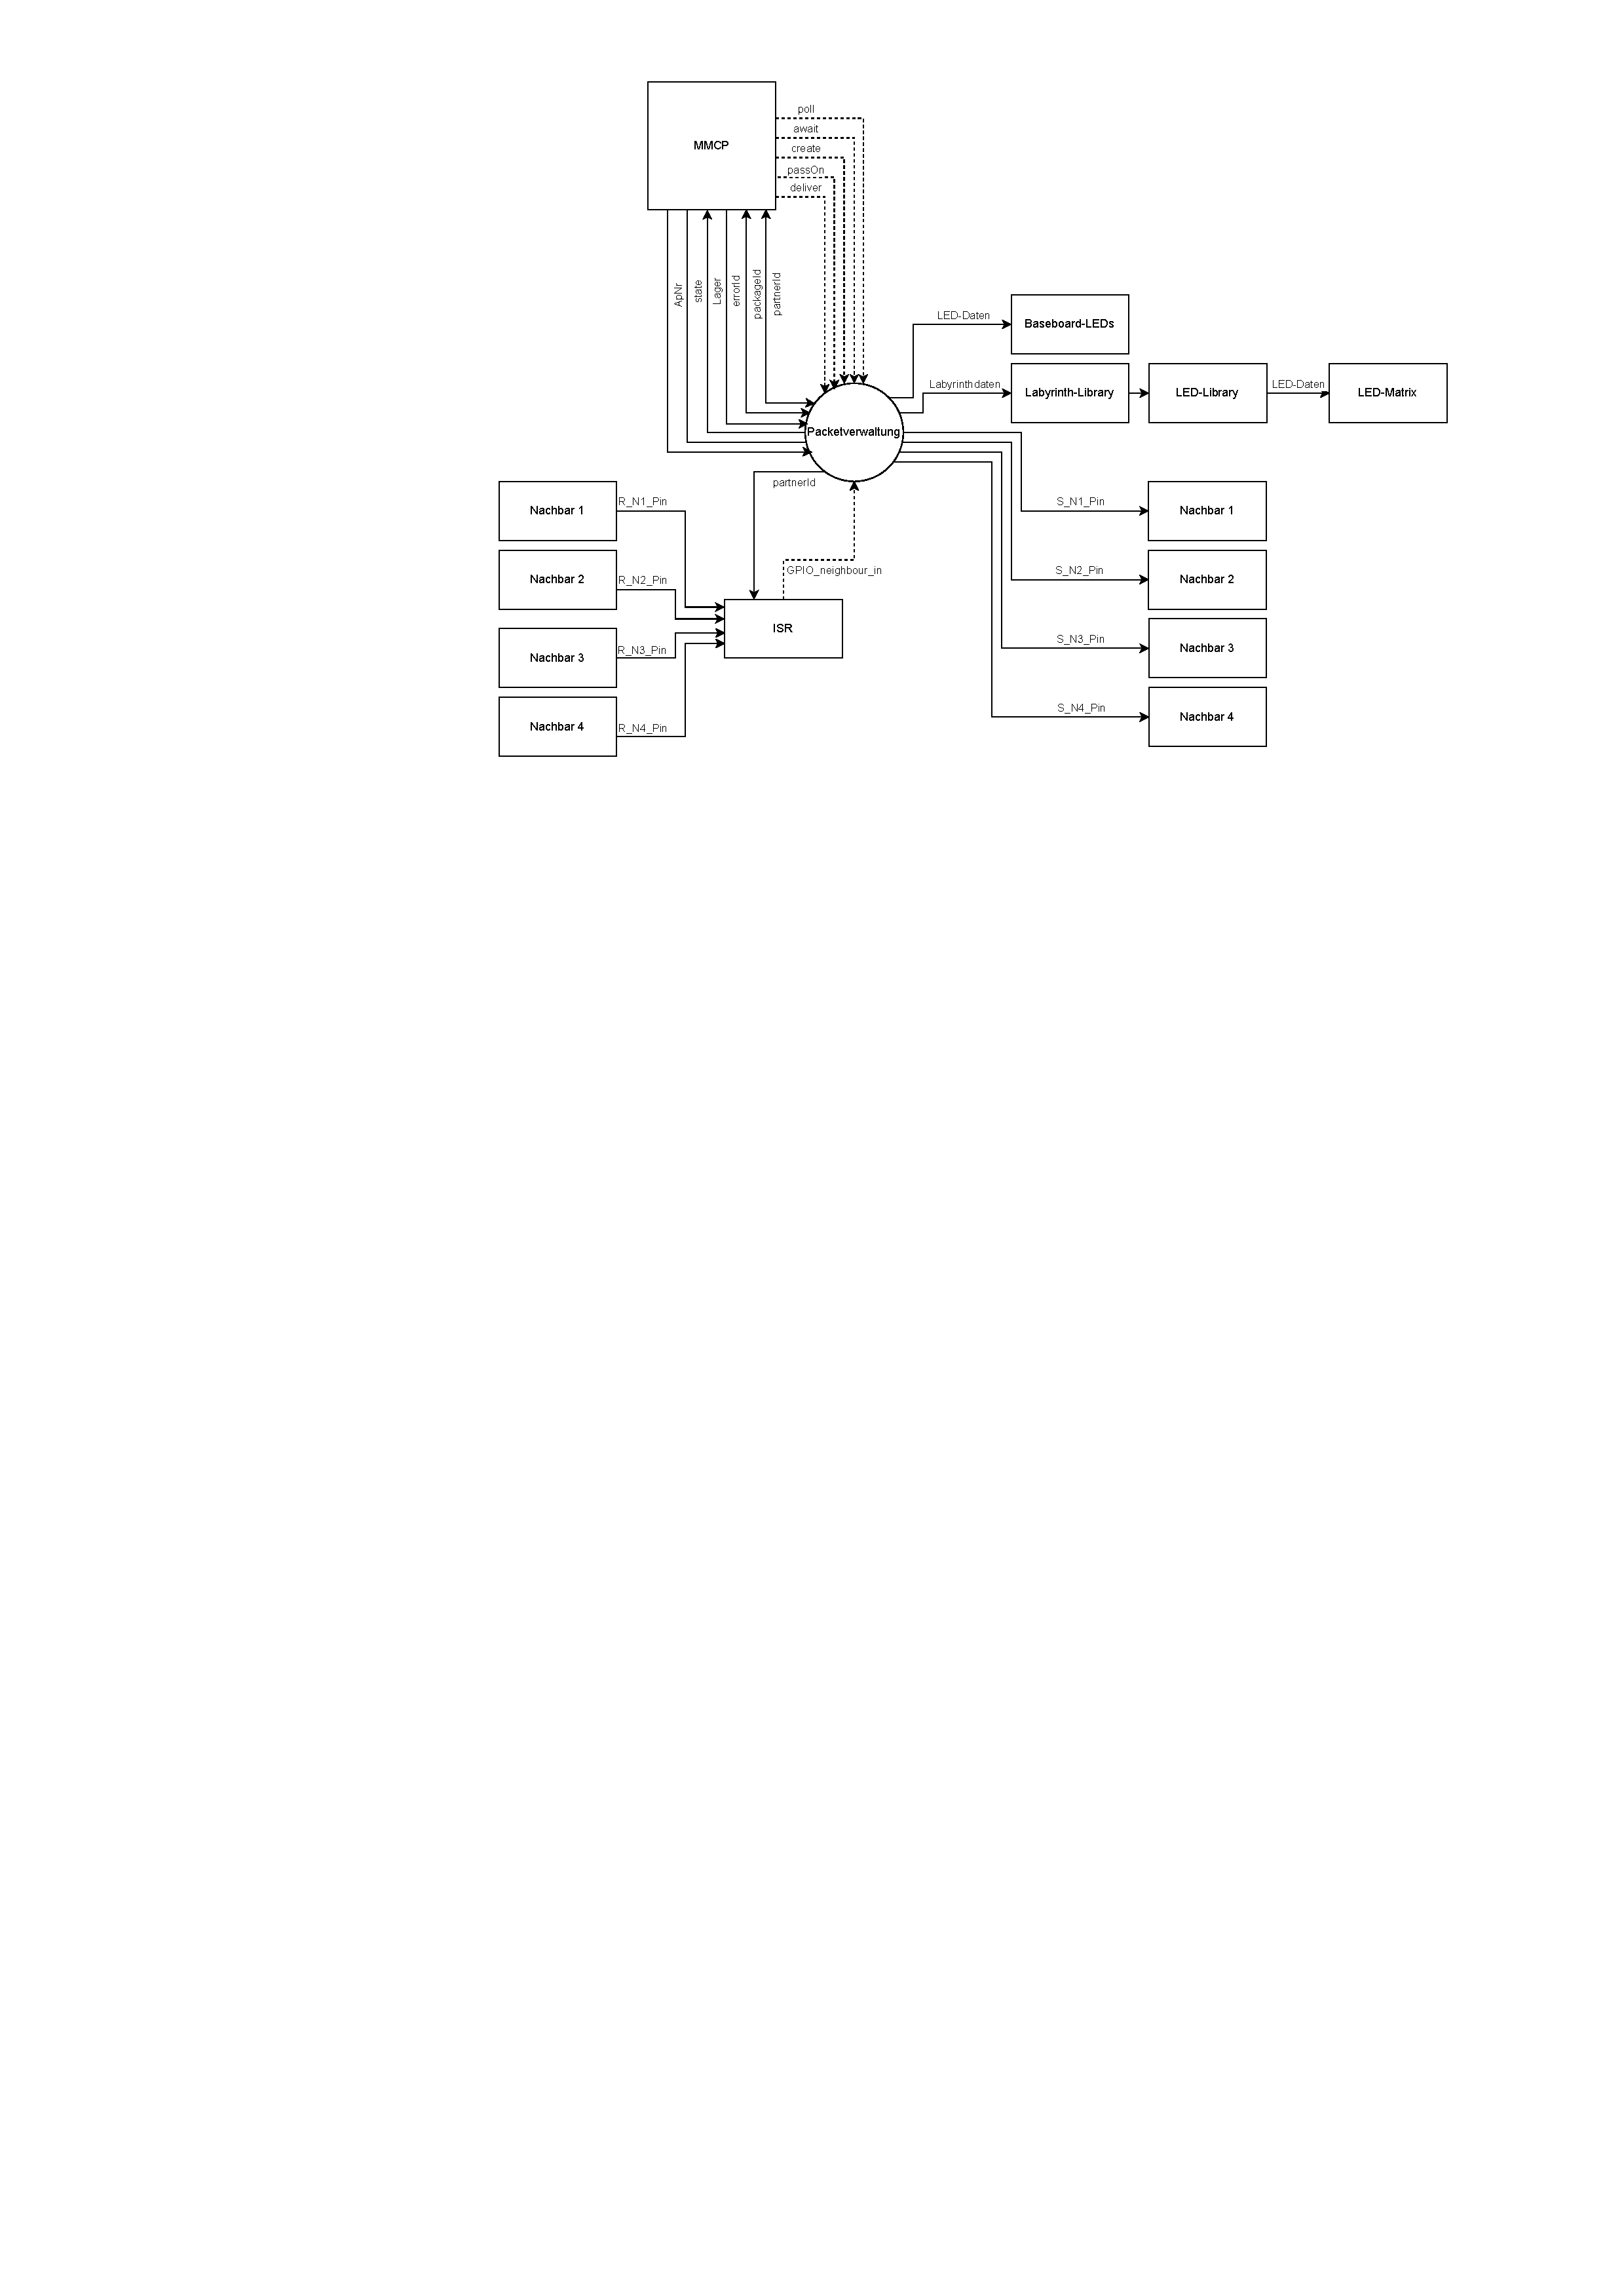
\includegraphics[page=1,width=0.9\textwidth]{pdfs/Kontextdiagramm.pdf} 
    \caption{Kontextdiagramm}
    \label{fig:Kontextdiagramm}
\end{figure}

\subsection{Datenflussdiagramm}
\begin{figure}[H]
    \centering
    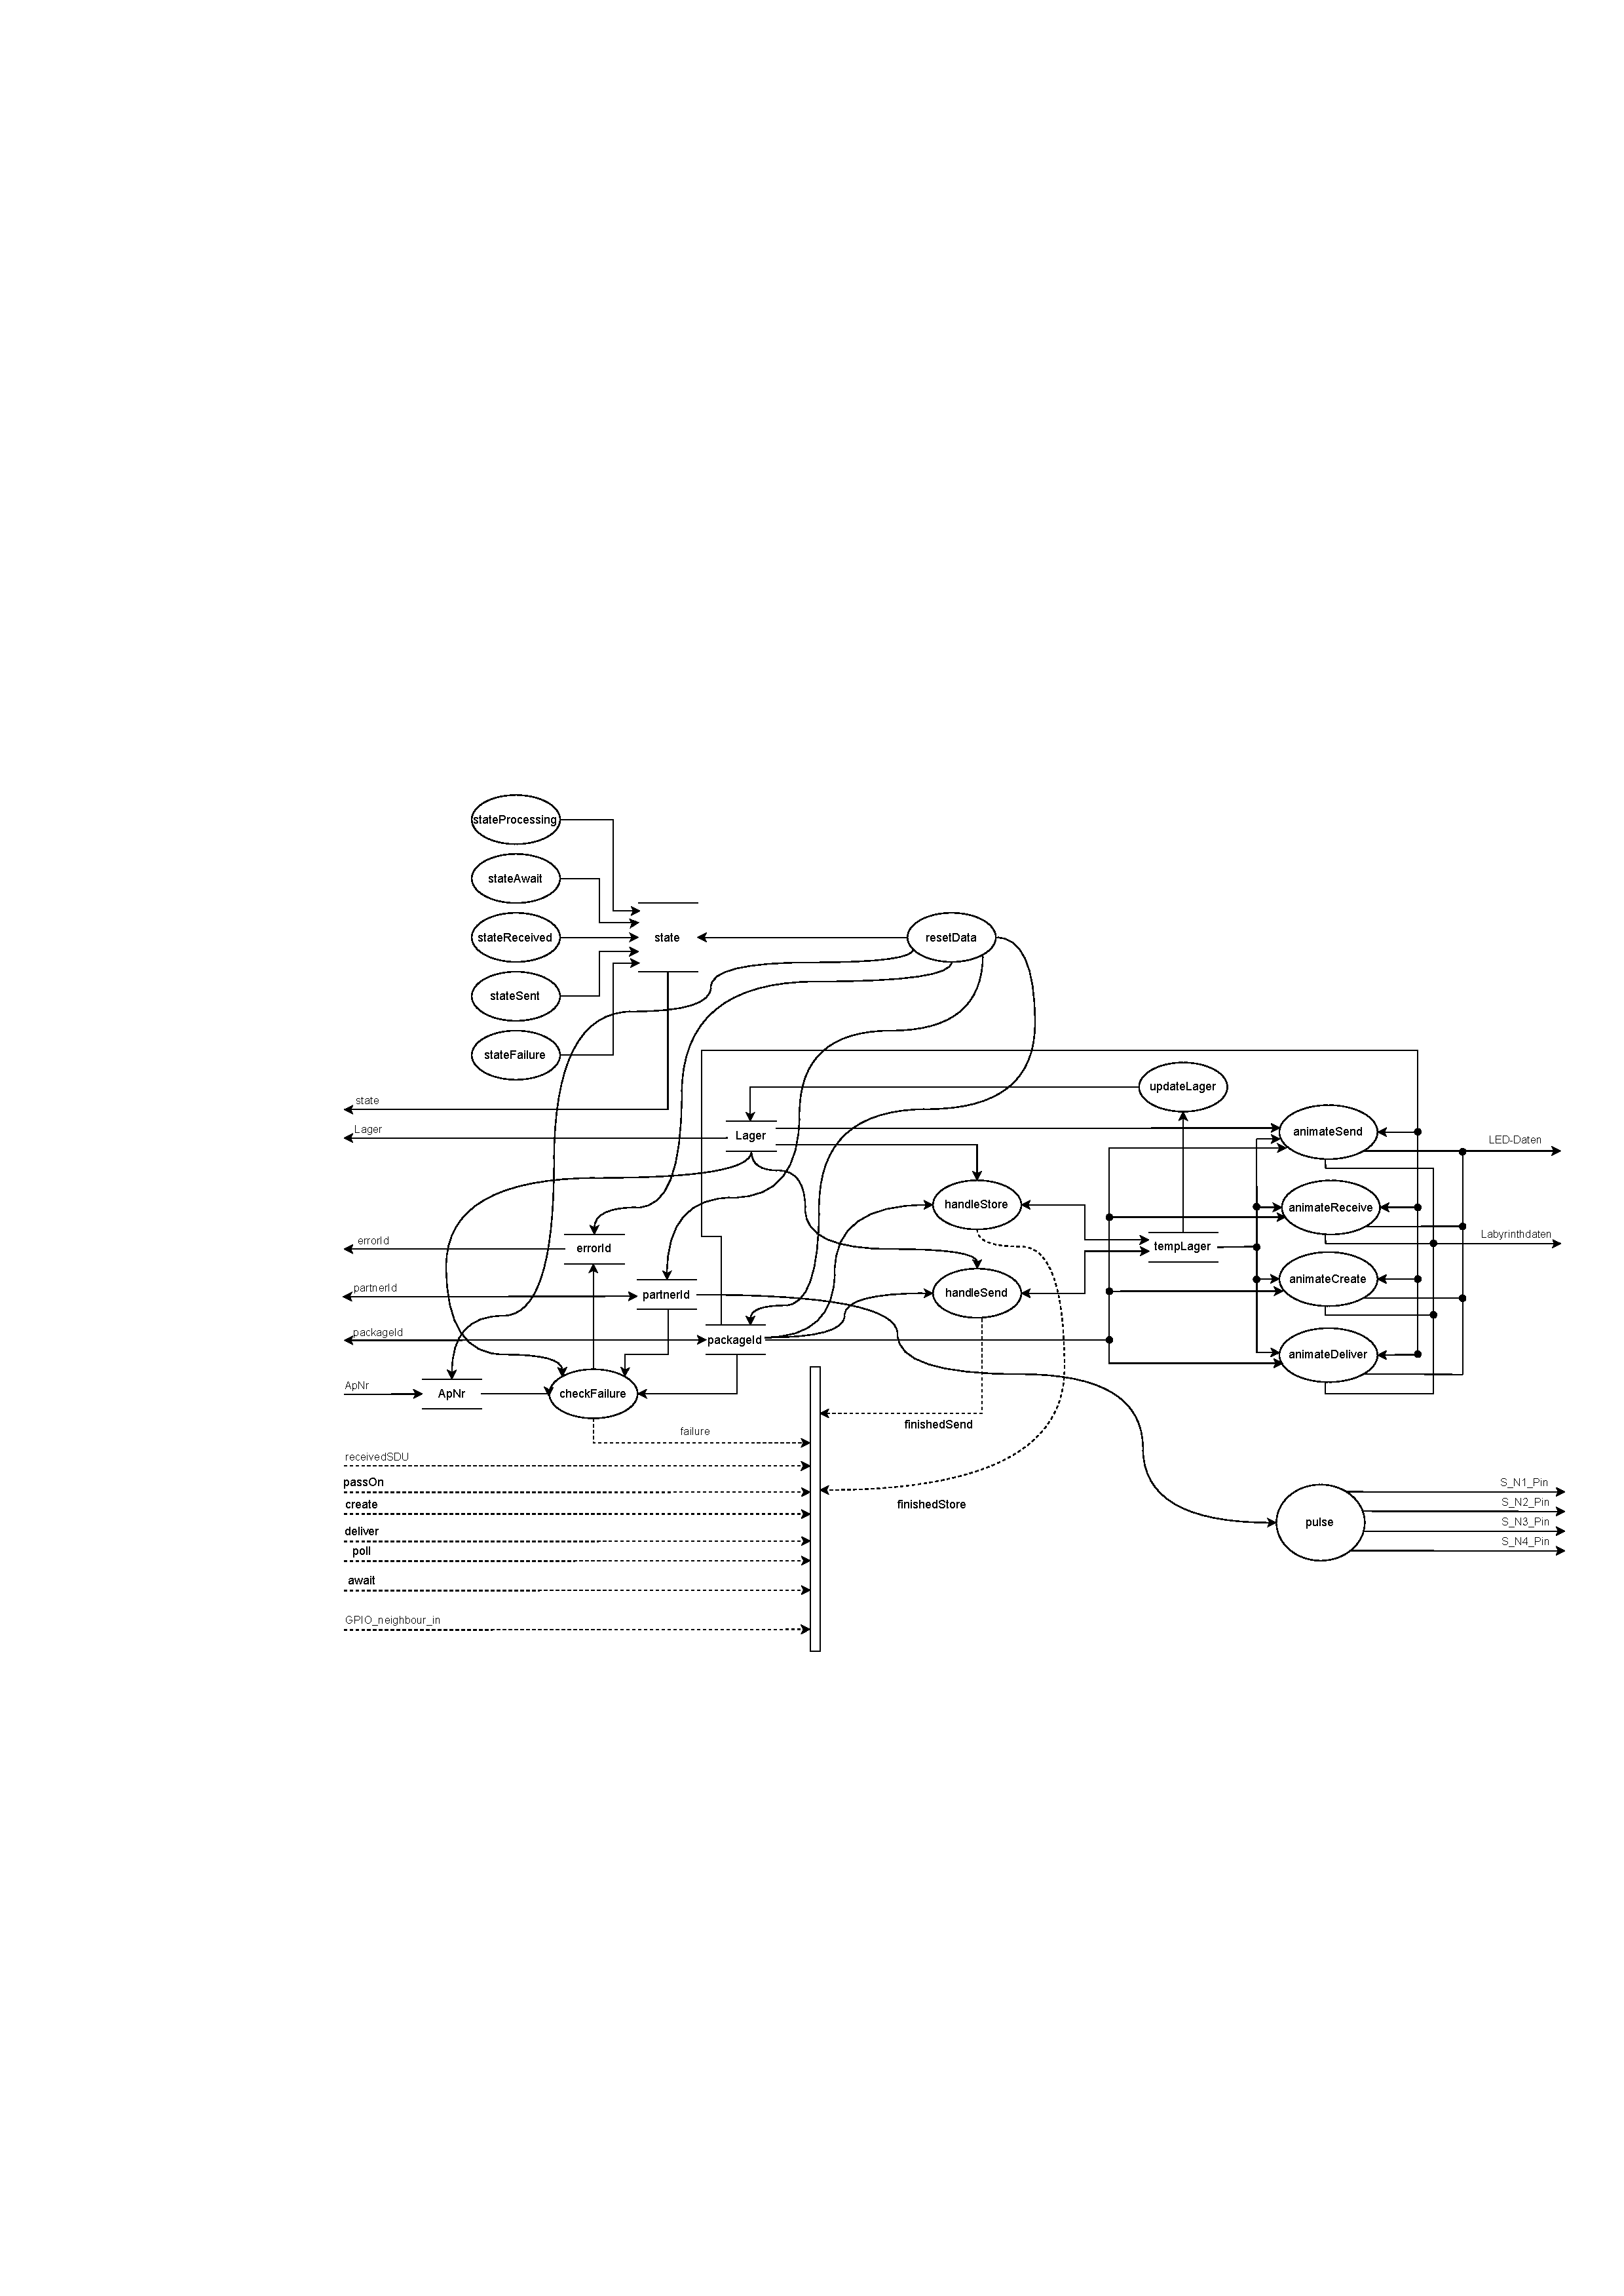
\includegraphics[page=1,width=\textwidth]{pdfs/Datenflussdiagramm.pdf} 
    \caption{Datenflussdiagramm}
    \label{fig:Datenflussdiagramm}
\end{figure}

\subsection{Zustandsübergangsdiagramm}
\begin{figure}[H]
    \centering
    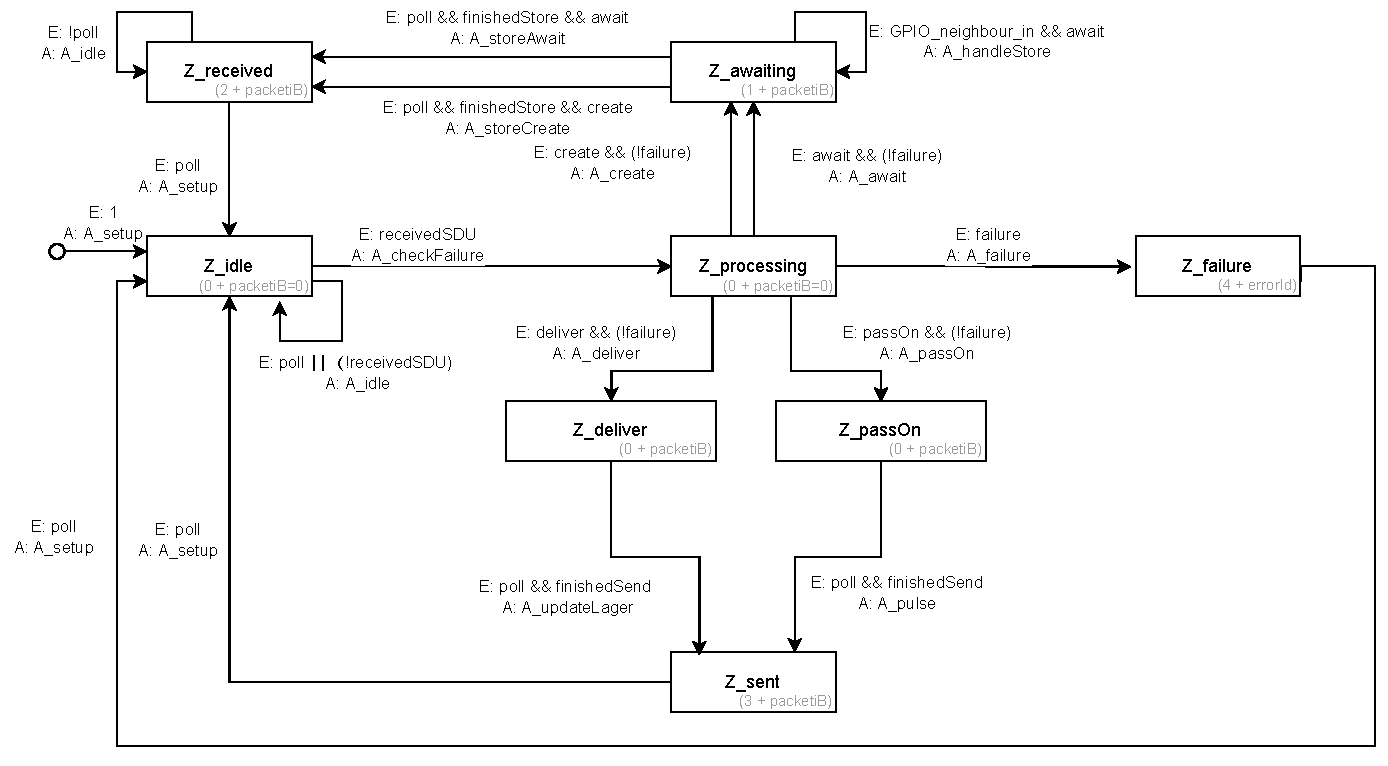
\includegraphics[page=1,width=0.85\textwidth]{pdfs/Zustandsuebergangsdiagramm.pdf} 
    \caption{Zustandsübergangsdiagramm}
    \label{fig:Zustandsuebergangsdiagramm}
\end{figure}

\subsection{Datenverzeichnis}
\begin{lstlisting}[style=CBlank]
DATA state = " uint_8 "
DATA errorId = " uint_8 "
DATA partnerId = " uint_8 "
DATA packageId = " uint_8 "
DATA Lager = " uint_8[6] "
DATA tempLager = " uint_8[6] "
DATA ApNr = " uint_8 "

DATA receive = " bool " * Kontrollfluss *
DATA passOn = " bool " * Kontrollfluss *
DATA create = " bool " * Kontrollfluss *
DATA deliver = " bool " * Kontrollfluss *
DATA poll = " bool " * Kontrollfluss *
DATA await = " bool " * Kontrollfluss *
DATA finishedSend = " bool " * Kontrollfluss *
DATA finishedStore = " bool " * Kontrollfluss *
DATA failure = " bool " * Kontrollfluss *
DATA receivedSDU = " bool " * Kontrollfluss *
DATA GPIO_neighbour_in = " bool " * Kontrollfluss *
\end{lstlisting}

\subsection{Minispezifikation}

\subsubsection*{stateProcessing}
Setzt \texttt{state} auf 0. Dieser Code steht für den Status \enquote{processing}, welcher dem Master über das MMCP-Protokoll zurückgemeldet wird.

\subsubsection*{stateAwait}
Setzt \texttt{state} auf 1. Dieser Code steht für den Status \enquote{awaiting}, welcher dem Master über das MMCP-Protokoll zurückgemeldet wird.

\subsubsection*{stateReceived}
Setzt \texttt{state} auf 2. Dieser Code steht für den Status \enquote{received}, welcher dem Master über das MMCP-Protokoll zurückgemeldet wird.

\subsubsection*{stateSent}
Setzt \texttt{state} auf 3. Dieser Code steht für den Status \enquote{sent}, welcher dem Master über das MMCP-Protokoll zurückgemeldet wird.

\subsubsection*{stateFailure}
Setzt \texttt{state} auf 4. Dieser Code steht für den Status \enquote{failure}, welcher dem Master über das MMCP-Protokoll zurückgemeldet wird.

\subsubsection*{handleStore}
Speichert Paket mit der Nummer \texttt{packageId} im \texttt{tempLager} Array an der ersten freien Stelle \texttt{i}, wo \texttt{tempLager[i] == 0} gilt.

\subsubsection*{handleSend}
Löscht Paket mit der Nummer \texttt{packageId} aus dem \texttt{tempLager} Array, setzt also an der Stelle \texttt{i} des Pakets \texttt{tempLager[i] = 0}.

\subsubsection*{updateLager}
Kopiert den \texttt{tempLager} Array zum \texttt{Lager} Array.

\subsubsection*{animateSend}
Senden eines Paketes auf der LED-Anzeige des Baseboards animieren und den Inhalt von \texttt{Lager} mit vorgeschriebenen Farben für jede verschiedene Paketnummer \texttt{packageId} darstellen. Ruft Funktionen der Labyrinth-Library auf, welche das Labyrinth generieren, lösen und anschließend den Weg der Paketdrohne durch das Labyrinth animieren. Genauere Beschreibung der Funktionen in \ref{Labyrinth}.

\subsubsection*{animateReceive}
Empfangen eines Paketes auf der LED-Anzeige des Baseboards animieren und den Inhalt von \texttt{Lager} mit vorgeschriebenen Farben für jede verschiedene Paketnummer \texttt{packageId} darstellen. Ruft Funktionen der Labyrinth-Library auf, welche das Labyrinth generieren, lösen und anschließend den Weg der Paketdrohne durch das Labyrinth animieren. Genauere Beschreibung der Funktionen in \ref{Labyrinth}.

\subsubsection*{animateCreate}
Erstellen eines Paketes auf der LED-Anzeige des Baseboards animieren und den Inhalt von \texttt{Lager} mit vorgeschriebenen Farben für jede verschiedene Paketnummer \texttt{packageId} darstellen.

\subsubsection*{animateDeliver}
Löschen eines Paketes auf der LED-Anzeige animieren des Baseboards und den Inhalt von \texttt{Lager} mit vorgeschriebenen Farben für jede verschiedene Paketnummer \texttt{packageId} darstellen.

\subsubsection*{pulse}
Gibt eine steigende Flanke mit der Dauer 1 ms auf dem zu \texttt{partnerId} korrespondierenden GPIO-Pin aus. Die Zuordnung von Pins und Nachbarn ist als Konstante im Code realisiert.

\subsubsection*{checkFailure}
Überprüft den empfangenen Befehl auf logische Fehler und Ausführbarkeit. 
\\
Zuerst wird überprüft, ob \texttt{partnerId} ein bekannter Nachbar bzw. \texttt{0} ist. Ist dies nicht der Fall, so wird \texttt{errorId = 4} und \texttt{failure = TRUE} gesetzt. Die Liste der Nachbarn ist als Konstante im Code realisiert.
\\
Ist \texttt{ApNr == 42}, ein Paket soll also erstellt oder empfangen werden, wird überprüft, ob der \texttt{Lager} Array noch einen freien Platz \texttt{Lager[i] == 0} hat. Ist dies nicht der Fall, so wird \texttt{errorId = 2} und \texttt{failure = TRUE} gesetzt.
\\
Zudem wird überprüft, ob \texttt{packageId} bereits im \texttt{Lager} Array vorhanden ist. Ist dies der Fall, so wird \texttt{errorId = 1} und \texttt{failure = TRUE} gesetzt.
\\
Ist \texttt{ApNr == 43}, ein Paket soll gelöscht oder weitergeleitet werden, wird überprüft, ob der \texttt{packageId} im \texttt{Lager} Array existiert. Ist dies nicht der Fall, so wird \texttt{errorId = 3} und \texttt{failure = TRUE} gesetzt.
\\
Zuletzt wird überprüft, ob \texttt{packageId} eine gültige Paketnummer (zwischen einschließlich 1 und 16) ist. Ist dies nicht der Fall, so wird \texttt{errorId = 5} und \texttt{failure = TRUE} gesetzt.

\subsubsection*{resetData}
Setzt \texttt{packageId}, \texttt{partnerId}, \texttt{errorId} und \texttt{ApNr} auf \texttt{0}. Setzt \texttt{rceeive}, \texttt{passOn}, \texttt{create}, \texttt{deliver}, \texttt{poll}, \texttt{await}, \texttt{failure}, \texttt{finishedStore}, \texttt{finishedSend}, \texttt{receivedSDU} auf \texttt{FALSE}.

\subsection{Prozessaktivierungstabelle}
\begin{table}[htbp]
  \centering
  \rowcolors{1}{white}{lightgray}
  \begin{tabular}{|*{18}{c|}}
    \hline
    \rotatebox{45}{  Aktion/Prozess} &
    \rotatebox{90}{stateProcessing} &
    \rotatebox{90}{stateAwait} &
    \rotatebox{90}{stateReceived} &
    \rotatebox{90}{stateSent} &
    \rotatebox{90}{stateReceived} &
    \rotatebox{90}{stateFailure} &
    \rotatebox{90}{handleStore} &
    \rotatebox{90}{handleSend} &
    \rotatebox{90}{updateLager} &
    \rotatebox{90}{animateSend} &
    \rotatebox{90}{animateReceive} &
    \rotatebox{90}{animateCreate} &
    \rotatebox{90}{animateDeliver} &
    \rotatebox{90}{pulse} &
    \rotatebox{90}{checkFailure} &
    \rotatebox{90}{resetData} \\
    \hline
    A\_setup        & 2 & & & & & & & & & & & & &  & &1\\
    A\_deliver      & 1 & & & & & & & 2 & & & & & & & &\\
    A\_passOn       & 1 & & & & & & & 2 & & & & & & & &\\
    A\_failure      & & & & & & 1 & & & & & & & & & &\\
    A\_pulse        & & & & 4 & & & & & 3 & 1 & & & & 2 & &\\
    A\_updateLager  & & & & 3 & & & & & 2 & & & & 1 & & &\\
    A\_await        & & 1 & & & & & & & & & & & & & &\\
    A\_create       & & 1 & & & & & 2 & & & & & & & & &\\
    A\_handleStore  & & & & & & & 1 & & & & & & & & &\\
    A\_storeAwait    & & & 3 & & & & & & 2 & & 1 & & & & &\\
    A\_storeCreate   & & & & & 3 & & & & 2 & & & 1 & & & &\\
    A\_checkFailure  & 2 & & & & & & & & & & & & & & 1 &\\
    A\_idle          & & & & & & & & & & & & & & & &\\
    \hline
  \end{tabular}
  \caption{Prozessaktivierungstabelle}
  \label{tab:Prozessaktivierungstabelle}
\end{table}